\documentclass[journal]{IEEEtran}
% *** CITATION PACKAGES ***
% \usepackage[style=ieee]{biblatex} 
% \bibliography{example_bib.bib}    %your file created using JabRef

% *** MATH PACKAGES ***
\usepackage{amsmath}
% URL LINK
\usepackage{hyperref}
% *** PDF, URL AND HYPERLINK PACKAGES ***
\usepackage{url}
% correct bad hyphenation here
\hyphenation{op-tical net-works semi-conduc-tor}
\usepackage{graphicx}  %needed to include png, eps figures
\usepackage{float}  % used to fix location of images i.e.\begin{figure}[H]

\usepackage[utf8]{inputenc}

\usepackage{titling}

% CODE STYLE
\usepackage{listings}
\usepackage{xcolor}

%New colors defined below
\definecolor{codegreen}{rgb}{0,0.6,0}
\definecolor{codegray}{rgb}{0.5,0.5,0.5}
\definecolor{codepurple}{rgb}{0.58,0,0.82}
\definecolor{backcolour}{rgb}{0.95,0.95,0.92}

%Code listing style named "mystyle"
\lstdefinestyle{mystyle}{
  backgroundcolor=\color{backcolour},   commentstyle=\color{codegreen},
  keywordstyle=\color{magenta},
  numberstyle=\tiny\color{codegray},
  stringstyle=\color{codepurple},
  basicstyle=\ttfamily\footnotesize,
  breakatwhitespace=false,         
  breaklines=true,                 
  captionpos=b,                    
  keepspaces=true,                 
  numbers=left,                    
  numbersep=5pt,                  
  showspaces=false,                
  showstringspaces=false,
  showtabs=false,                  
  tabsize=2
}
%"mystyle" code listing set
\lstset{style=mystyle}
% END CODE STYLE


\begin{document}
% paper title
\title{Predicting Ratings of Users on Yelp}
% author names 
\author{Zihe Wang (zw2624), Di Ye (dy2404)\\ Ziyao Zhang (zz2583), Yinhe Lu (yl4372)}
% The report headers
\markboth{IEORE 4571: Personalization, December 2019}
{Shell \MakeLowercase{\textit{et al.}}: Bare Demo of IEEEtran.cls for IEEE Journals}
% make the title area
% \maketitle
% Abstract
\IEEEtitleabstractindextext{%
\begin{abstract}
    This project aims to predict the rating of a user to a certain business. We used the public Yelp dataset as our dataset. We performed three tasks, evaluating how well the models predict the rating by using accuracy metrics, comparing the ranking of the business to see whether the predicted rank is aligned with the true ranking order, and measuring the model performance on different segmentation of users and businesses. We used item-based collaborative filtering, and Non-negative Matrix Factorization (NMF) as our baseline models. Then we explored three more complex models for comparison of results, which are Factorization Machine (FM), Neural Collaborative filtering (NCF) and Wide \& Deep (W\&D) model. Our experiments suggested that FM and W\&D model perform particular better compared to the baseline model and NCF.
\end{abstract}

\begin{IEEEkeywords}
Recommendation System, Collaborative Filtering, Deep Learning, Neural Network, Personalization
\end{IEEEkeywords}}
% make the title area
\maketitle
\IEEEdisplaynontitleabstractindextext

\IEEEpeerreviewmaketitle


\section{Introduction}

\IEEEPARstart{Y}{ELP} connects people to great local businesses. To help people find great local businesses, Yelp engineers have developed an excellent search engine to sift through over 171 million cumulative reviews that have been contributed.


Our project used Yelp's dataset at \href{https://www.yelp.com/dataset/challenge}{\underline{Yelp Data Challenge}}. In order to recommend a business to a user well, the predicted rating of this user to businesses is important. To address this issue, we have experimented on Factorization Machine, Neural Collaborative Filtering and Wide \& Deep model. We have also explored model performances on different businesses based on popularity and users with different level of prolificness. Moreover, in recommendation task, not only an accurate predicted rating is important, the relative order of the business in prediction is also important. In this paper, we aimed to explore these tasks in our models. We used an item-based collaborative filtering and Non-negative Matrix Factorization model as our baseline model. 

Summary of the objectives:
\begin{enumerate}
    \item How close our prediction is to the actual rating
    \item Whether the predicted ranking of businesses is the same as the actual ranking
    \item How do our models perform on different segmentation of users and businesses
\end{enumerate}


\section{Data Preparation \& Exploration}

\subsection{Data Overview}
The Yelp dataset is a subset of Yelp’s businesses, reviews, and user data for use in personal, educational, and academic purposes. The dataset is available as JSON files which can be access \href{https://www.yelp.com/dataset}{\underline{here}}. In our project, we used review.json, user.json and business.json in the dataset. Review.json contains full review text data including the user\_id that wrote the review and the business\_id the review is written for.

\subsubsection{Review}
Review.json file is our main focus in this project. In review.json file, some important features we care about are user\_id, business\_id, star rating, and date/timestamp. A data sample and its description is shown below. 


\begin{lstlisting}[language=Python, caption=Review Data Example]
{
    // string, 22 character unique user_id, maps to the user in user.json
    "user_id": "Ha3iJu77CxlrFm-vQRs_8g",
    
    // string, 22 character business_id, maps to business in business.json
    "business_id": "tnhfDv5Il8EaGSXZGiuQGg",
    
    // integer, star rating
    "stars": 4,
    
    // string, date formatted YYYY-MM-DD
    "date": "2016-03-09"
}
\end{lstlisting}

\begin{figure}
\begin {center}
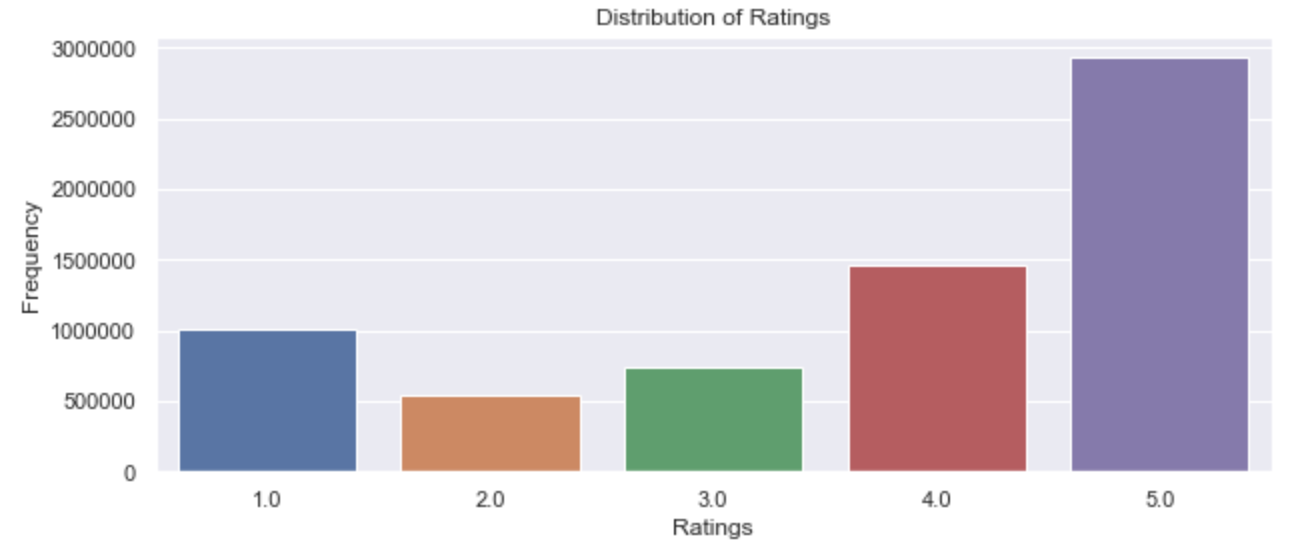
\includegraphics[width=0.45\textwidth]{images/review_rating_bar_chart.png}
\caption{Users' Review Ratings}
\label{fig:review_rating}
\end {center}
\end{figure}


\subsubsection{Users}
We also explored user information as supplemental information to see whether we can understand the Yelp data better. The listing of the users' information what we think is useful to explore users' aspect. We used some of the features in the models.

\begin{lstlisting}[language=Python, caption=Users Data Example]
{
    // string, 22 character unique user id, maps to the user in user.json
    "user_id": "Ha3iJu77CxlrFm-vQRs_8g",

    // array of strings, an array of the friends of the user as user_ids
    "friends": [
        "wqoXYLWmpkEH0YvTmHBsJQ",
        "KUXLLiJGrjtSsapmxmpvTA",
        "6e9rJKQC3n0RSKyHLViL-Q"
    ],

    // integer, number of useful votes sent by the user
    "useful": 21,

    // integer, number of funny votes sent by the user
    "funny": 88,

    // integer, number of cool votes sent by the user
    "cool": 15,

    // integer, number of fans the user has
    "fans": 1032,

    // array of integers, the years the user was elite
    "elite": [
        2012,
        2013
    ],
    // float, average rating of all reviews
    "average_stars": 4.31,

    // integer, number of hot compliments received by the user
    "compliment_hot": 339,

    // integer, number of more compliments received by the user
    "compliment_more": 668,

    // integer, number of cute compliments received by the user
    "compliment_cute": 62,

    // integer, number of cool compliments received by the user
    "compliment_cool": 91
}
\end{lstlisting}

\subsubsection{Business}

Since Business.json provides lots of information about the stores, we focused on name of the restaurant, their locations and their ratings and review counts. We tried to find out about top name/brand of the stores and see their popularity by looking at their review counts. From {\it Figure~\ref{fig:review_rating}}, we noticed that the majority of the stores have average rating around 3.5 - 4. We can see from {\it Figure~\ref{fig:top_name_store}} that we have lots of top stores in the dataset, such as Starbucks, McDonald's and Subway, which are open nationwide. We also believe that the store brand can also affect the popularity and rankings of the store.

\begin{lstlisting}[language=Python, caption=Business Data Example]
{
    // string, 22 character unique string business_id
    "business_id": "tnhfDv5Il8EaGSXZGiuQGg",

    // string, the name of the business
    "name": "Garaje",

    // string, the city
    "city": "San Francisco",

    // string, 2 character state code, if applicable
    "state": "CA",

    // float, star rating, rounded to half-stars
    "stars": 4.5,
    // integer, number of reviews
    "review_count": 1198
}
\end{lstlisting}

\begin{figure}
\begin {center}
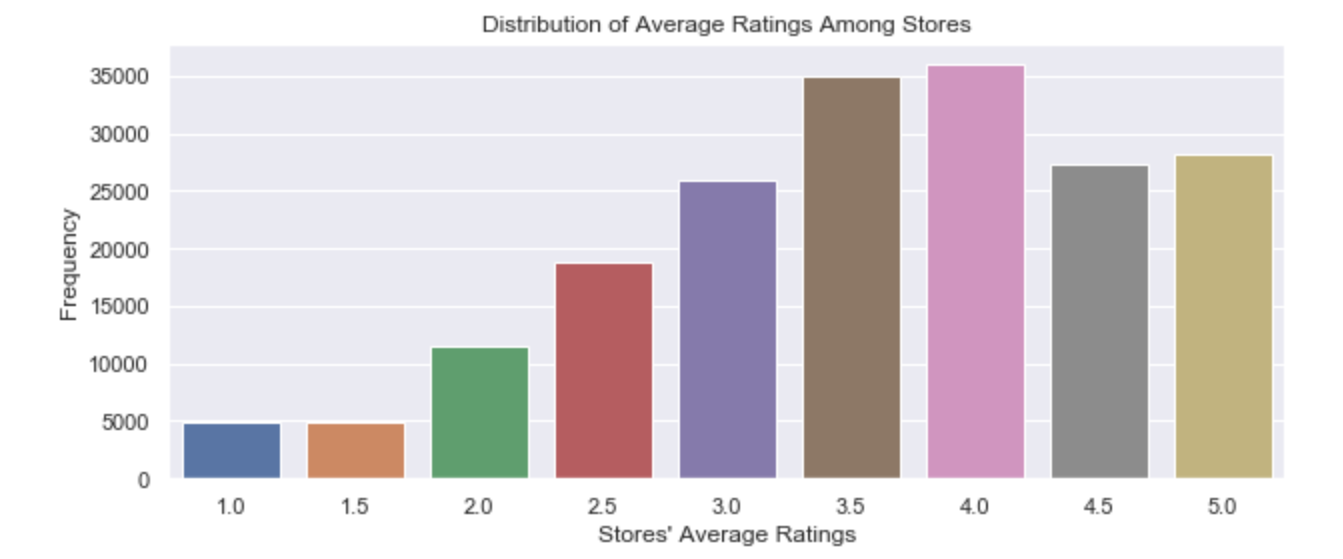
\includegraphics[width=0.45\textwidth]{images/stores_average_ratings.png}
\caption{Users' Review Ratings}
\label{fig:review_rating}
\end {center}
\end{figure}

\begin{figure}
\begin {center}
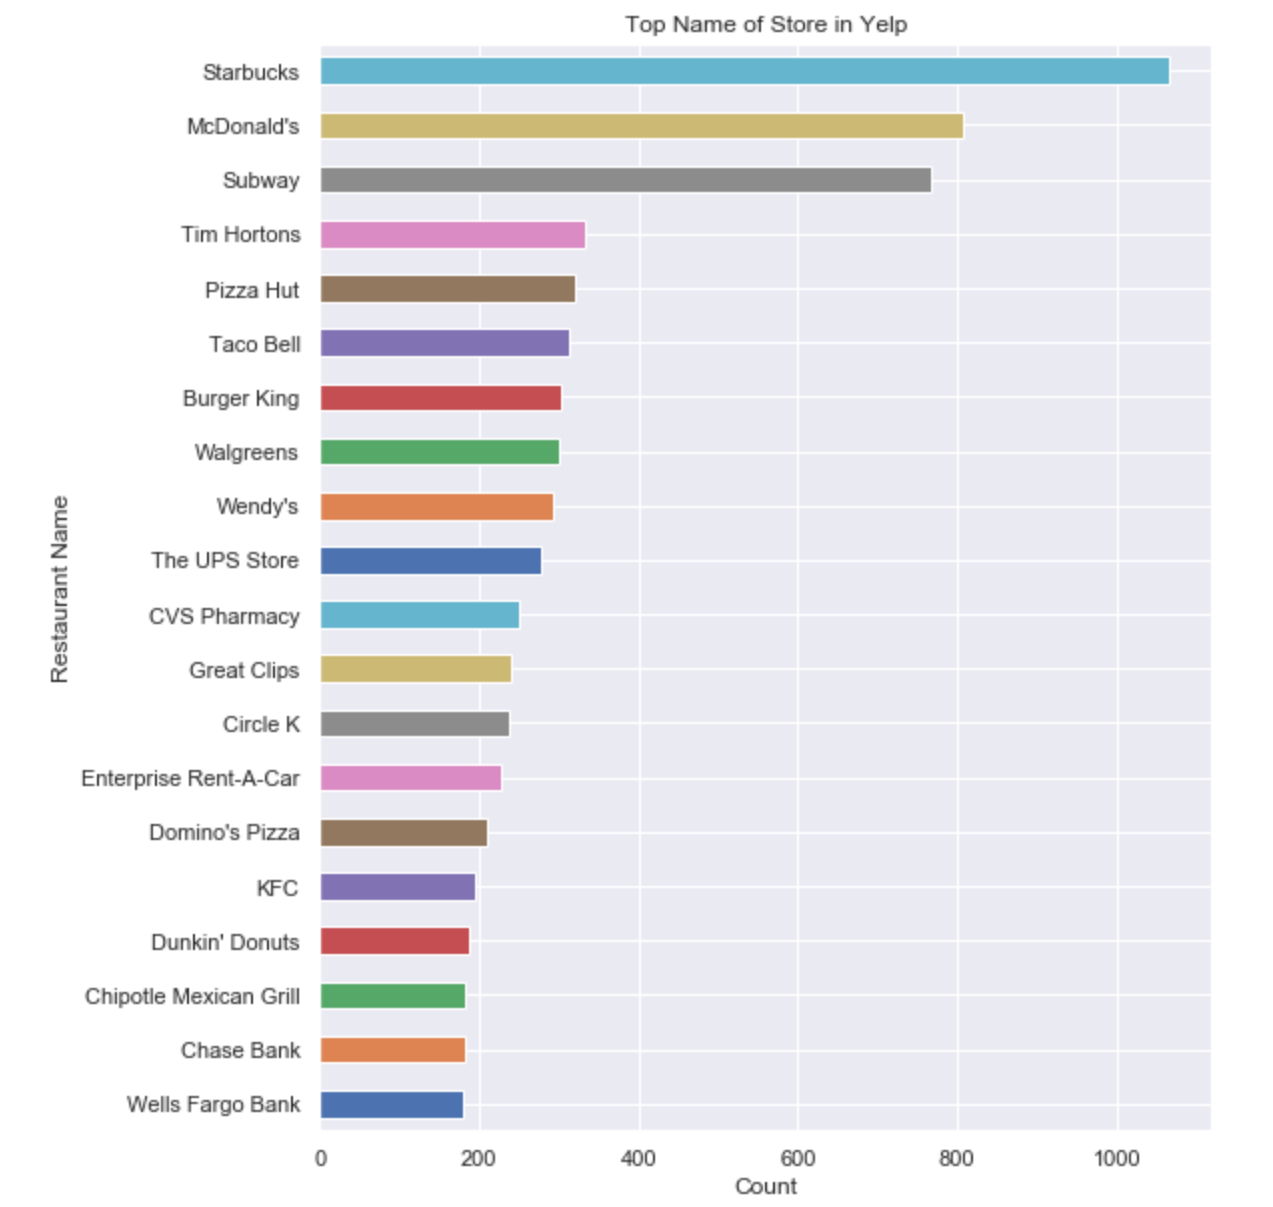
\includegraphics[width=0.45\textwidth]{images/top_name_in_yelp.png}
\caption{Top Name of Store in Yelp}
\label{fig:top_name_store}
\end {center}
\end{figure}

\subsubsection{Tip}
Tip.json contains tips written by a user on a business. Tips are shorter than reviews and tend to convey quick suggestions. We created the word cloud for both the reviews and tips for data exploratory analysis. The tip's word cloud gives us much more information compared to the review's word cloud, because tip contains more precise and succinct reviews for the store. Therefore, we only put the tip's word cloud here in {\it Figure~\ref{fig:tip_wordcloud}}. We can see that the word cloud for tips conveys some information about the rating of a store. Most of the words are either positive or neutral, which matches with the distribution of the ratings. 

\begin{figure}
\begin {center}
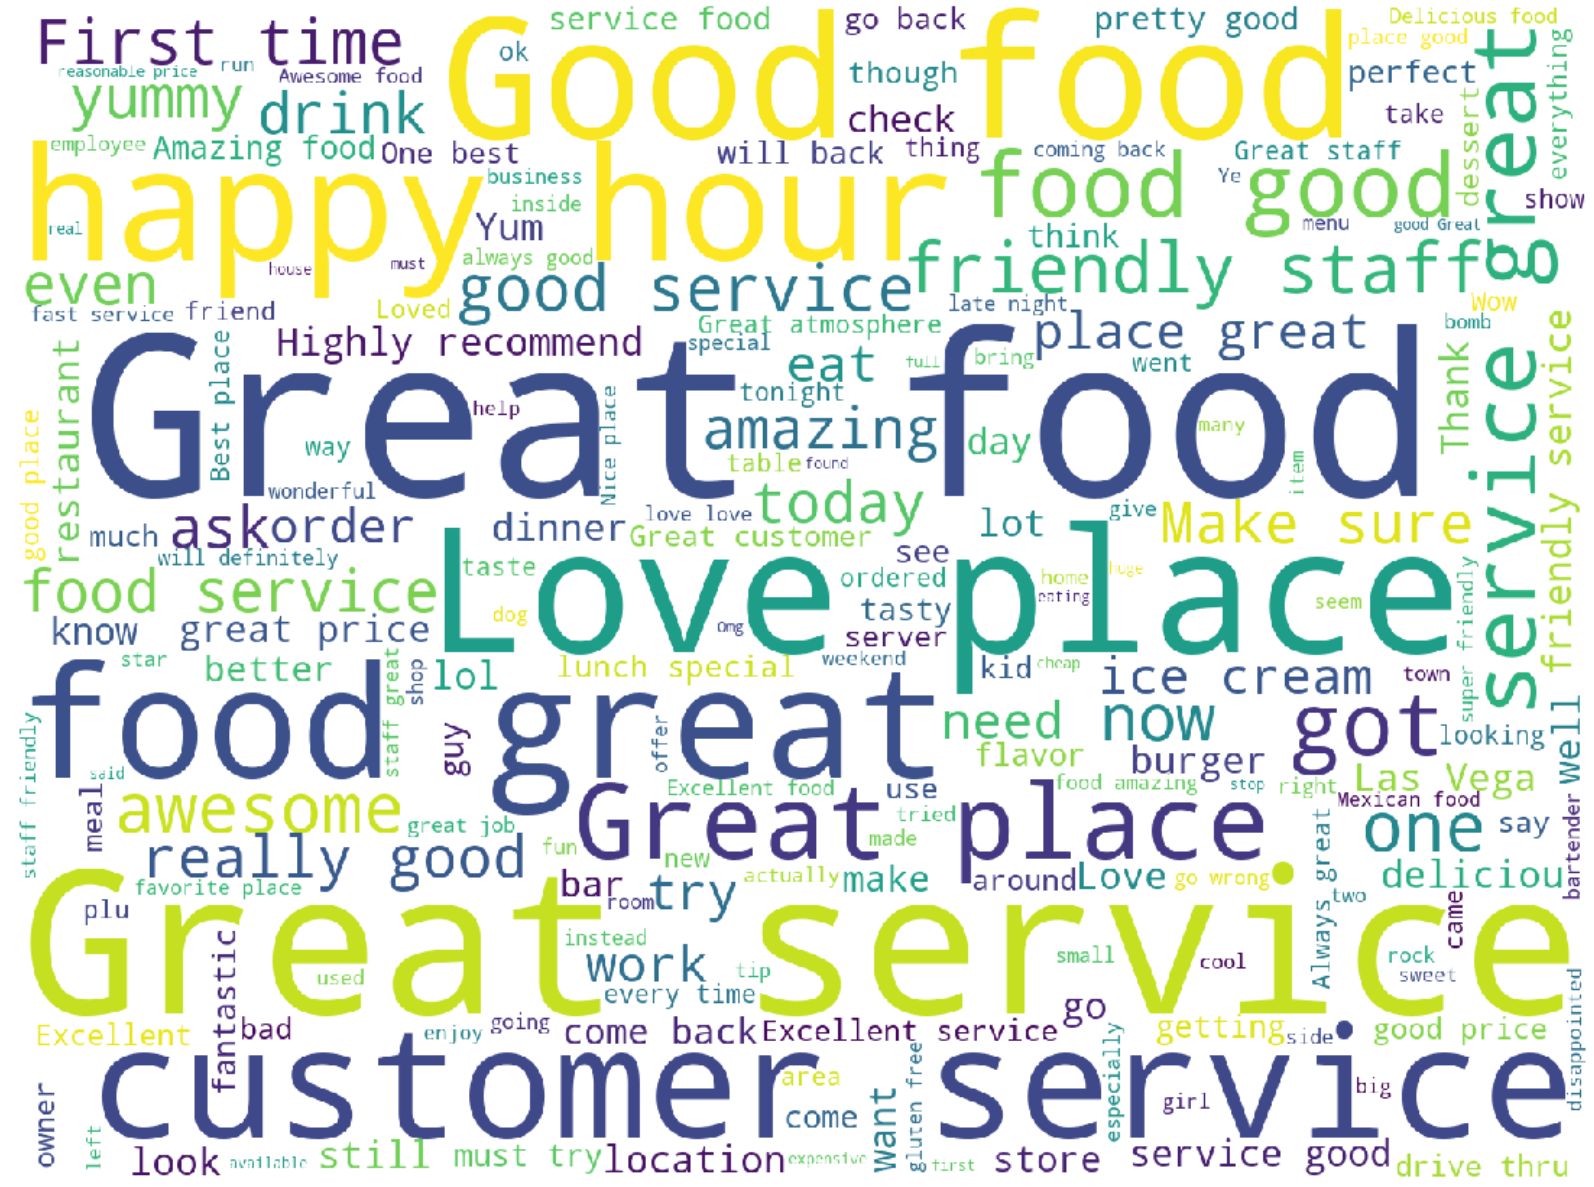
\includegraphics[width=0.45\textwidth]{images/tip_wordcloud.png}
\caption{Word Cloud for Tips Written by users on businesses}
\label{fig:tip_wordcloud}
\end {center}
\end{figure}

\subsection{Data Sampling}

In the original review dataset, we have 1637138 unique user\_id and 192606 unique business\_id. First, we need to build a dataset that we are going to use for training and testing. We filtered out the businesses that appear less than twice in the whole dataset. Then we  took the users with 5 or more reviews as active users. We only focused on analyzing the data of the active users. After this initial step of data filtering, we have 281365 unique user\_id and 172970 unique business\_id left.

We constructed three sets of dataset.

\begin{enumerate}
    \item {\bf Large Dataset}: We are able to train the three more complex models on the full dataset after the initial filtering steps mentioned above. So we constructed a larger dataset to train these three models and compared the results. We first hold out the last review of each user as the test set. Then, we randomly took another two reviews from each user for the purpose of comparison of ranking. Later, we evaluate the metrics for both the constructed whole test set and the test set with the last review only.
    \item {\bf Small Dataset}: Due to the computational time and space constrain, we were not able to run the large dataset on baseline models. Therefore, we sampled a smaller dataset so that we could run these two models smoothly. We randomly picked 20000 unique users from the full dataset. This smaller dataset contians 258564 reviews and 72323 unique businesses. We have also trained our three advanced models on this smaller dataset for the purpose of comparison of results. Similarly, we evaluate the metrics for both the constructed whole test set and the test set with the last review only.
    \item {\bf Data Segmentation}: The third objective of this project is to explore model performances on different segmentation of users and businesses. We segmented users and businesses into three levels: unpopular, mid-popular and popular. We first took the median of the frequency of user/business. The user/business that has frequency less than median will be counted as an unpopular user/business. Next, any user/business that has frequency between the median and the mean of the frequency column is counted as mid-popular user/business. Last, the user/business that has frequency more than the mean is counted as a popular user/business. For here, frequency of a user means the number of reviews that user wrote before, and frequency of a business mean the number of times that business has been rated before. Please note that for here, a 'popular' user means a 'prolific' user, we call them 'popular' just for simplicity.
\end{enumerate}



\section{Methodology}

\subsection{Baseline Model}
We used baseline bias model, neighborhood-based method and Non-negative Matrix Factorization (NMF) as our baseline models.

\subsubsection{Baseline Bias Model}
We use a baseline model for comparing results. The model uses the baseline estimate for given user and item. \footnote{https://surprise.readthedocs.io/en/stable/basic\_algorithms.html}

$$\hat \mu_i = b_{ui} = \mu + b_u + b_i$$
If user $u$ is unknown, then the bias $b_u$ is assumed to be zero. The same applies for item $i$ with $b_i$

\subsubsection{Item-Based Neighborhood Model}
   \\Item-based  neighborhood  models allow for natural explanations to the user. Item-based  methods  can  be  more  stable  than  user-based methods, since there is likely more overlap between businesses than users. An extra business is added less  frequently  than  users  to  total  dataset,  so  it could be less computational expensive.
For Item-based Neighborhood Models, similarities need to be computed between businesses. Three similarity function variants are tried in our project: Cosine, Pearson baseline, Pearson. 


{\bf RawCosine}($i, j$) = $$\frac{\sum_{k \in I_u \cap I_v} r_{uk} r_{vk}}{\sqrt{\sum_{k \in I_u \cap I_v}r_{uk}^2} \sqrt{\sum_{k \in I_u \cap I_v}r_{vk}^2}}$$

{\bf PearsonBaseline}($u, v$) = $$\frac{\sum_{k \in I_u \cap I_v} (r_{uk} - b_{uk})(r_{vk}-b_{vk})}{\sqrt{\sum_{k \in I_u \cap I_v}(r_{uk} - b_{uk})^2} \sqrt{\sum_{k \in I_u \cap I_v}(r_{vk} - b_{vk})^2}}$$

{\bf Pearson}($u, v$) = $$\frac{\sum_{k \in I_u \cap I_v} (r_{uk} - \mu_u)(r_{vk}-\mu_v)}{\sqrt{\sum_{k \in I_u \cap I_v}(r_{uk} - \mu_u)^2} \sqrt{\sum_{k \in I_u \cap I_v}(r_{vk} - \mu_v)^2}}$$

The predicted rating $\hat r_{uj}$ of user $u$ for target item $t$ is as follows:
$$\hat r_{uj} = \mu_u + \frac{\sum_{v \in P_u(j)} Sim(u,v) (r_{vj} - \mu_v)}{\sum_{v \in P_u(j)} |Sim(u, v)|}$$

where $P_u(j)$ is the peer set of $k$ closest neighbors to user $u$ that have a rating for item $j$.

\subsubsection{Model-based CF: Non-negative Matrix Factorization}
Non-negative Matrix Factorization (NMF) has a high level of interpretation in understanding the user-item interactions. The optimization formulation in NMF is shown below:
$$Minimize J = \frac{1}{2}||R-Q^TP||^2$$ with  $$P_i, Q_i \ge 0$$ 
at each iteration, the matrices are updated:
$$p_{uf} \leftarrow p_{uf} \cdot \frac{\sum_{i \in I_u} q_{if}
\cdot r_{ui}}{\sum_{i \in I_u} q_{if} \cdot \hat{r_{ui}} +
\lambda_u |I_u| p_{uf}}$$\\
$$q_{if} \leftarrow q_{if} \cdot \frac{\sum_{u \in U_i} p_{uf}
\cdot r_{ui}}{\sum_{u \in U_i} p_{uf} \cdot \hat{r_{ui}} +
\lambda_i |U_i| q_{if}}$$\\
We used the following parameter to adjust our method:
\begin{itemize}
    \item rank – The number of factors. 
    \item epoch – The number of iteration of the SGD procedure. 
    \item $p_u$ – The regularization term for user factor.
    \item $q_i$ – The regularization term for item factor.
\end{itemize}

\subsection{Factorization Machine}
In Steffen Rendle's paper, the author introduces factorization machines (FMs), a state of the art solution to problems including multiple entity types. They are similar to other collective approaches in that they allow for multiple relationships between multiple entities, but differ in at least a few ways, including:
\begin{itemize}
    \item FMs use a clever feature representation to cast factorization as a regression, classification, or ranking problem.
    \item In addition to relations between entity types, FMs allow for interaction terms for items within a single entity type.
    \item FMs can be defined such that they act like, or mimic, other techniques like SVD++. 
\end{itemize}

Feature generation for factorization machines one-hot-encodes users and businesses, and uses the rating variable itself as a target variable, much like regression or classification.

In our project, we not only considered user id, business id as features, but also consider other features that have been provided to us, such as the city of the restaurant, the stars of the business, average rating of all reviews a user gave. We have also create new features, such as the number of friends a user has.

\subsection{Neural Collaborative Filtering}
We also tried the Neural Collaborative Filtering framework (He X., 2011) to further explore the potential of the generalized matrix factorization. The structure of the framework is shown in {\it Figure~\ref{fig:ncf}}.  
\begin{figure}
 \center
  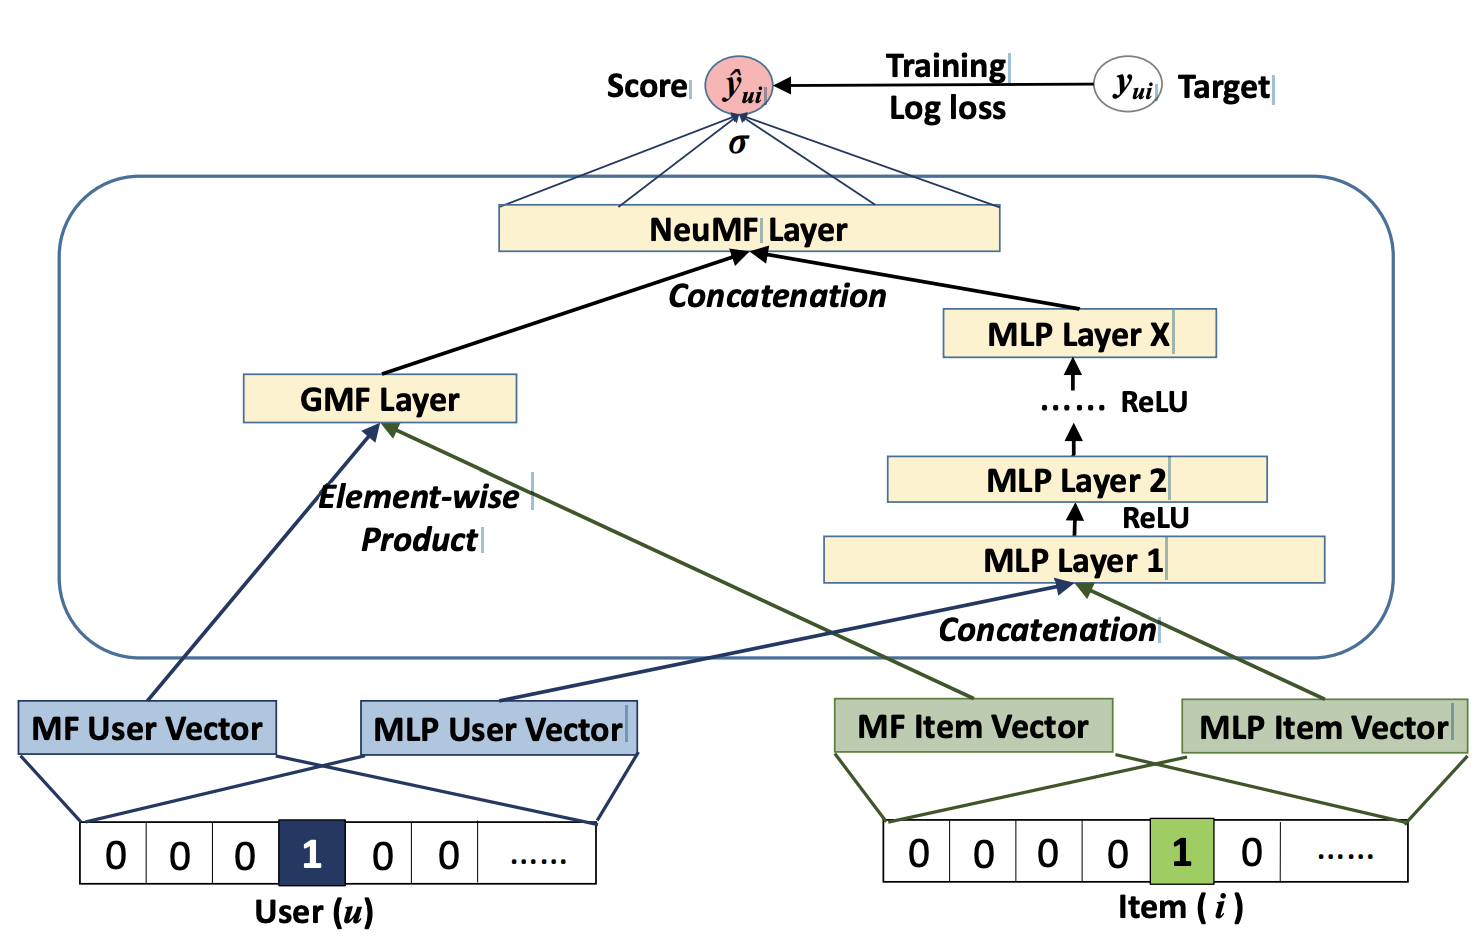
\includegraphics[width=0.45\textwidth]{images/NeuralCF_structure.png}
  \caption{Neural Collaborative Filtering Model}
  \label{fig:ncf}
\end{figure}

The idea is that: first, we use fully connected layers to convert our sparse input matrix (user and item) into two embedding layers. Then, we built two paths for the inputs: one is called \textbf{GMF}, another one is called \textbf{MLP}.
\subsubsection{GMF}
GMF is the generalized matrix factorization. 
\begin{equation}
    \hat{y_{ui}} = a(h^T(p_u*q_i))
    \label{equation:GMF}
\end{equation}
where $a$ is the activation function and $h$ is the edge weights of the output layer. We can introduce non-linearity by changing activation function and learn the weights through $h$.

\subsubsection{MLP}
MLP is Multi-Layer Perceptron. It contains multiple hidden layers and the purpose of passing user and item vectors into this network is to learn the non-linear interaction between user and item. 

The outputs of GMF and MLP are concatenated in a final fully connected layer to get the output.


\subsection{Wide \& Deep}
In the project, we used a Wide \& Deep Learning framework to achieve both memorization and generalization in one model, by jointly training a linear model component and a
neural network component as shown in {\it Figure~\ref{fig:wide_deep}}.  

\subsubsection{Wide Models}
Wide models are similar to logistic regression.

Equation~\ref{equation:wide_model1}. 
\begin{equation}
    y = w^Tx + b
    \label{equation:wide_model1}
\end{equation}
One of the most important transformations is the cross-product transformation, defined as 

\begin{equation}
    \phi_k(x) = \prod_{i=1}^{d} x_i^{c_{ki}} \; c_{ki} \in \{0, 1\}
    \label{equation:wide_model2}
\end{equation}
where $c_ki$ is a booklean variable that is 1 if the $i$th feature is part of the $k$-th transformation $\phi_k$, and 0 otherwise.

\subsubsection{Deep Models}

\begin{equation}
    a^{(l+1)} = f(W^{(l)}a^{(l)}+b^{(l)})
    \label{equation:deep_model}
\end{equation}
where $l$ is the layer number and $f$ is the activation function, often rectified linear units (ReLUs). $a^{(l)}$, $b^{(l)}$, and $W^{(l)}$ are the activations, bias, and model weights at $l$-th layer.

Wide \& Deep model combines both models and trains on the combination of loss of these two models.

% FIGURE SAMPLE
% TO CITE THIS FIGURE: “Figure~\ref{fig:wide_deep}”
\begin{figure*}
 \center
  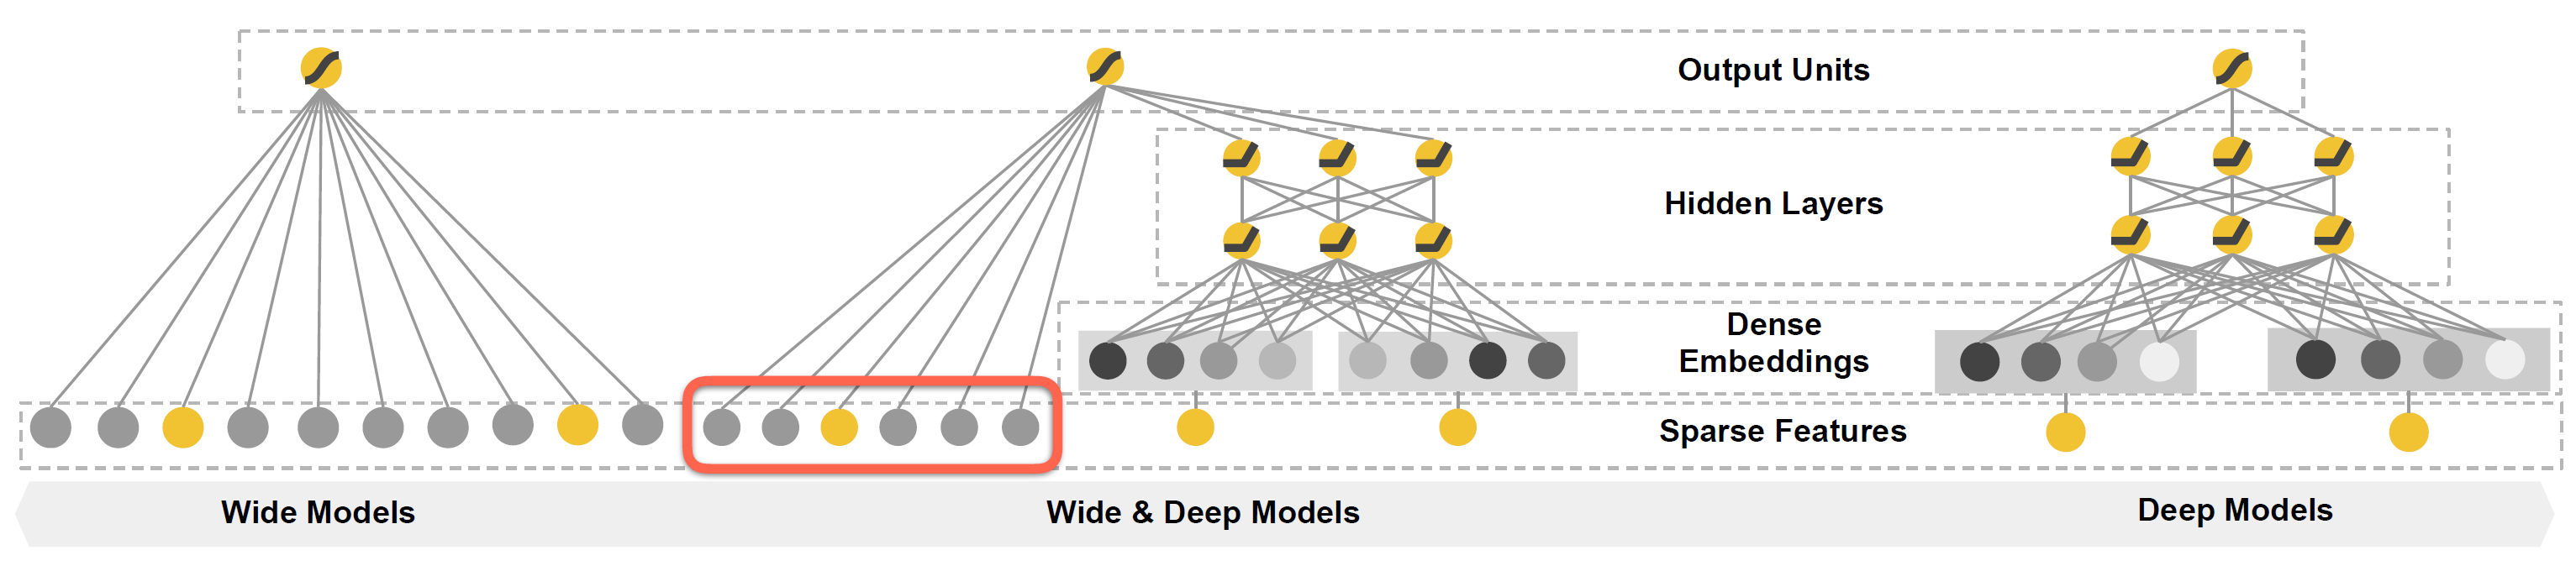
\includegraphics[width=\textwidth]{images/wide_deep.png}
  \caption{Wide \& Deep Model}
  \label{fig:wide_deep}
\end{figure*}

% FIGURE SAMPLE
% TO CITE THIS FIGURE: “Figure~\ref{fig:ecg}”
% \begin{figure}
% \begin {center}
% 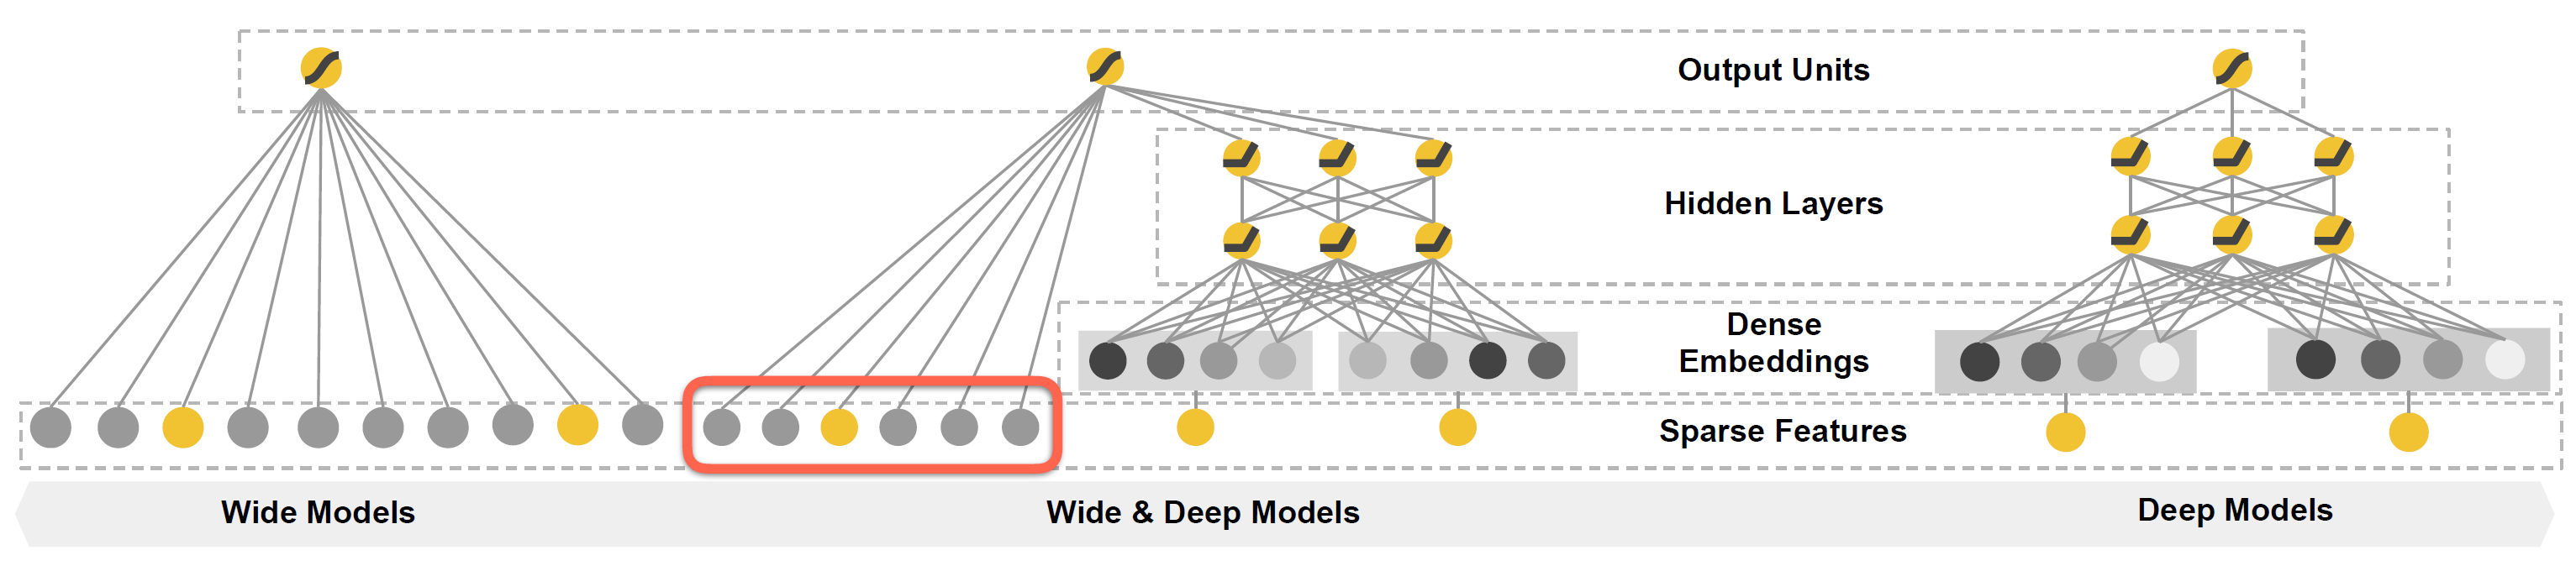
\includegraphics[width=0.45\textwidth]{images/wide_deep.png}
% \caption{Illustrations, graphs, and photographs may fit across both columns, if necessary. Your artwork must be in place in the article.}
% \label{fig:ecg}
% \end {center}
% \end{figure}






\section{Evaluation Metrics}

\subsection{Accuracy Metrics}

Next, we need to determine how good is our model. In our project, we used the root mean squared error ($RMSE$) to be our evaluation metrics.

We define $r_{uj}$ to be the value of the rating of the entry $(u, j)$ for user $u$'s rating on item $j$ in the test set, and $\hat r_{uj}$ be the predicted rating of the entry $(u,j)$.The error is given by $e_{uj} = \hat r_{uj} - r_{uj}$.The set $E$ corresponds to the held out entries in the hold-out methods.
$$RMSE = \sqrt \frac{{sum_{(u,j) \in E}e_{uj}^2}}{|E|}$$

This measurement can tell us how well our model predicted ratings. $RMSE$ is a good measurement when we choose to consider the effect of outliers.

\subsection{User Coverage}
Since there are three ratings for each user in the test set, except using $RMSE$ as the accuracy metric, we can evaluate the result of our model using the ranking order of the predictions. For instance, if the order of the predicted rating of the businesses in the test set is the same order of the true rating of the businesses in the test set, then this user will be counted as a well-recommended user. The order agreement means that the model can perfectly predict the ranking of the businesses despite the accuracy of the rating itself. After we define what is to be called a well-recommended user, then the user-coverage is the number of well-recommended users divided by the total number of users.
$$ UC = \frac{\# Well \; recommended \; Users}{\# Total \; Users}$$


% \bigskip
\bigskip

\section{Training Details And Results}
\subsection{Baseline Model}
For the neighborhood-based method, we tuned on the number of nearest neighbor $k$ and three similarity measures. We used gridsearch and cross-validation to search the best combination of parameters. For the similarity equation, we tried with cosine, pearson-baseline, and pearson equations. For the neighborhood size, we tested seven different $k$ values (5, 15, 25, 35, 45). We calculated $RMSE$ for each searching epoch, we used $RMSE$ to decide which parameter is the best parameter for the model. The result shows k=5 and pearson similarity will produce the lowest $RMSE$ value.

For the model-based method, we tuned on the number of factors and also regularization parameters. We used [10, 20, 30, 40, 50] for testing n$_$factors, [10, 50, 100] for testing n$_$epochs, [0.01, 0.05, 0.1] for testing reg$_$pu and [0.01, 0.05, 0.1] for testing reg$_$qi.  The lowest $RMSE$ value is produced when n$_$factors is  50, n$_$epochs is 50, reg$_$pu is 0.1 and reg$_$qi is  0.05.

\begin{figure}
\begin {center}
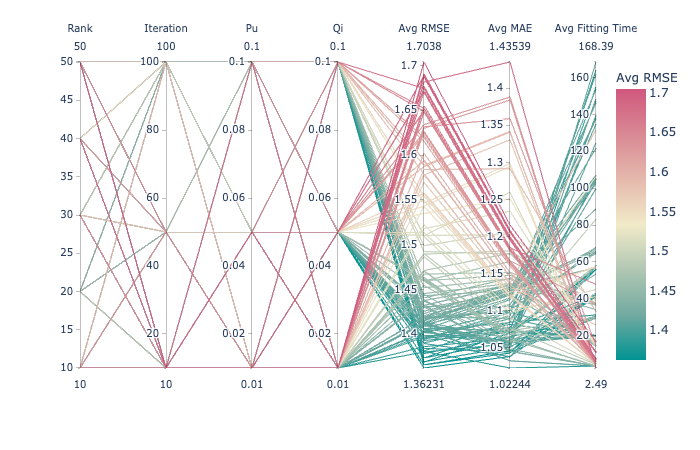
\includegraphics[width=0.45\textwidth]{images/nmfplot.png}
\caption{Parameter performance for NMF model}
\label{fig:nmfy}
\end {center}
\end{figure}
\begin{figure}
\begin {center}
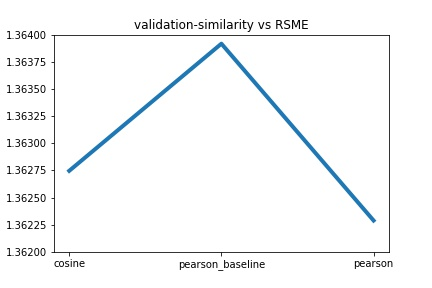
\includegraphics[width=0.45\textwidth]{images/similarity.jpg}
\caption{similarity measure parameter performance for KNN model}
\label{fig:nmfy}
\end {center}
\end{figure}
\begin{figure}
\begin {center}
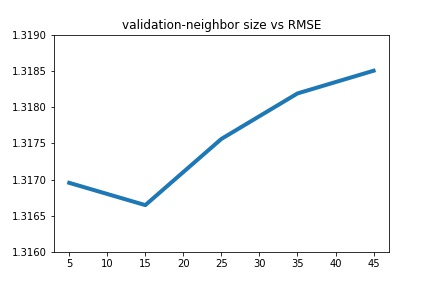
\includegraphics[width=0.45\textwidth]{images/neighbour.jpg}
\caption{number of neighbour parameter performance for KNN model}
\label{fig:nmfy}
\end {center}
\end{figure}

\subsection{Neural Collaborative Filtering}
We used python TensorFlow to build our models, and our major reference is Nipun Batra's blog. Since it is already a successfuly structure, the main thing we were tuning on this model is the non-linear part of the network. We tried different activation functions: leaky-Relu and Relu and each we fitted a model with 8 epochs. the result is shown below:
\begin{table}[H]  \centering
\caption{\label{} NCF model}
\label{my-label}
\begin{tabular}{c|ccccc}
\hline \hline
Activation      & RMSE      &  RMSE(last review)    & User Coverage \\ \hline
Relu            & 1.3910    & 1.4281                & 0.2145        \\ \hline
Leaky Relu      & 1.3880    & 1.4266                &  0.2147       \\ \hline
\end{tabular}
\end{table}
It turns out that the leaky relu is a better activation function on this dataset, and we chose it as our final activation function. 

We ran NCF on both the small and large dataset. From {\it Figure~\ref{fig:s_d_ncf_leaky}}, {\it Figure~\ref{fig:l_d_ncf_relu}} and {\it Figure~\ref{fig:l_d_ncf_leaky}}, we can see that the training loss is decreasing, the validation loss seems to be flat and has a slight increasing. We tried to avoid overfitting by adding regularization L2 and drop out layer. For the large dataset, we use fewer epoches due to running time. 
% TO CITE THIS FIGURE: “Figure~\ref{fig:ecg}”
\begin{figure}
\begin {center}
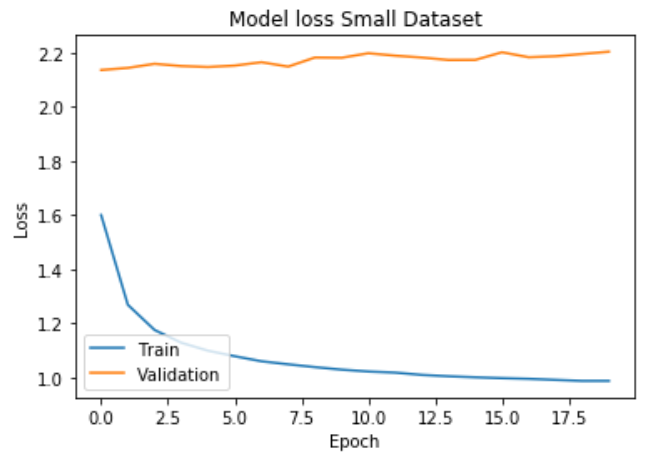
\includegraphics[width=0.45\textwidth]{images/small_dataset_model.png}
\caption{NCF Model Performance on Small Dataset}
\label{fig:s_d_ncf_leaky}
\end {center}
\end{figure}


\begin{figure}
\begin {center}
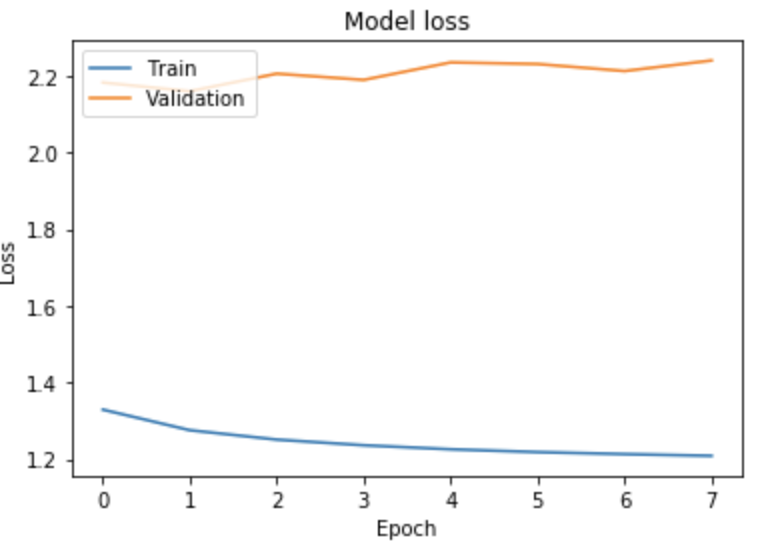
\includegraphics[width=0.45\textwidth]{images/relu.png}
\caption{NCF Model Performance on Large Dataset (ReLU)}
\label{fig:l_d_ncf_relu}
\end {center}
\end{figure}

\begin{figure}
\begin {center}
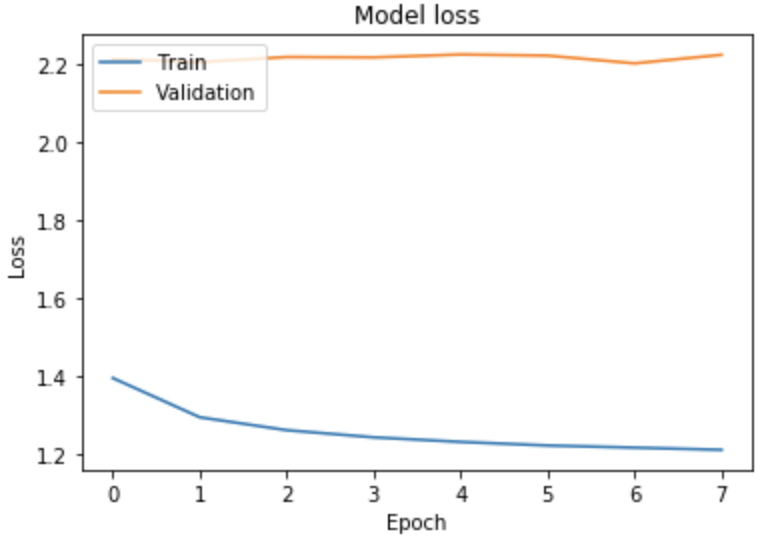
\includegraphics[width=0.45\textwidth]{images/leaky_relu.png}
\caption{NCF Model Performance on Large Dataset (Leaky ReLU)}
\label{fig:l_d_ncf_leaky}
\end {center}
\end{figure}


\subsection{Factorization Machine}
We used an open source Factorization Machine package[4] to implement our model. We have experimented with different combinations of features, for the conciseness of this paper, we would not list all the combination of features we have tried and only gave out the best results we got. The features that produced the results are `user id', `business id', `the stars of the business', `city' and `state'.
The number of iterations we chose is 15, since we have explored that more iterations will make the model suffer from overfitting. The initial learning rate is 0.001. These are the parameters that the model required to set before training. 

\subsection{Wide \& Deep}
The Wide \& Deep model contain two parts, a linear model and a deep learning model. Therefore, we have also explored the results by only using the Wide part and the Deep part separately. We have experimented with different combination of features that we used in training the model. To not redundant the report, we decide not to list all the combination of features we have tried but list the set of features that produce the best result we got. In the Wide part, we used `average stars',`useful review',`compliment more',`compliment cute',`number of friends',`city' and `state' after using hashing,`funny review',`cool review',`stars',`categories' and a cross feature of city and state. In the deep part, we used embedding layer of user and business of dimension of 32, and city of dimension 8, and `average stars', `compliment more', `stars', `useful', `funny', `cool', `fans', `compliment fun'. 

We have also tried with different number of hidden layers and hidden units. Moreover, we have tried with different loss functions. Inside the loss function, we have explored distinct learning rate, l1 regularization strength and l2 regularization strength. Again, we would not list every combination of choices we have experimented and only provide our final choices for the succinctness of this report. We chose to use ProximalAdagradOptimizer, with learning rate of 0.1, l1 regularization strength of 0.001, and l2 regularization strength of 0.001. The hidden units are [100,100,50,25]. We have also used batch normalization and set a dropout rate of 0.5. By using batch normalization and dropout, the model performed better. More discoveries and conclusions are written in the Conclusion and Discussion section.



\section{Results}
Below are all the results we got.

% TABLE SAMPLE
% TO CITE THIS TABLE "Table~\ref{table:Exps})"
\begin{table}[!ht] %[H]
\centering
\label{table:Exps}
\begin{tabular}{llll}
Models                  & $RMSE^1$  & $RMSE^2$  & User Coverage \\ \hline
Bias model(Baseline)    & 1.4782    & 1.5070    & 0.2057        \\
KNN(Baseline)           & 1.4981    & 1.5203    & 0.3059        \\
NMF(Baseline)           & 1.5016    & 1.5311    & 0.2341        \\
FM                      & 1.2111    & 1.2138    & 0.3216        \\
NCF                     & 1.4711    & 1.4387    & 0.2037        \\
W\&D(W\&D)              & 1.2711    & 1.2750    & 0.2955        \\
\end{tabular}
\caption{{\bf RMSE of Small Dataset}}
\end{table}

% \bigskip
% \bigskip

\begin{table}[!ht] %[H]
\centering
\label{table:Exps}
\begin{tabular}{llll}
Models      &  $RMSE^1$     & $RMSE^2$  &User Coverage \\ \hline
FM            & 1.2102      & 1.2154    & 0.2888    \\
NCF           & 1.3880      & 1.4266    & 0.2147    \\
W\&D(W\&D)    & 1.1984      & 1.1990    & 0.3059    \\
W\&D(Linear)  & 1.1644      & 1.1651    & 0.3045    \\
W\&D(DEEP)    & 1.3631      & 1.3643    & 0.2560    \\
\end{tabular}
\caption{{\bf RMSE of Large Dataset}}
\begin{tablenotes}
      \small
      \item In table II and III,
      \item $RMSE^1$ is the RMSE for only last rating of each user. 
      \item $RMSE^2$ is the RMSE for all ratings in the test set.
\end{tablenotes}
\end{table}

% \bigskip
% \bigskip

\begin{table}[!ht] %[H]
\centering
\label{table:Exps}
\begin{tabular}{llll}
Models &  $RMSE^1$ & $RMSE^2$ & $RMSE^3$\\ \hline
FM            & 1.2579   & 1.2455    & 1.1982\\
NCF           & 1.4468   & 1.3669    & 1.2739\\
W\&D(W\&D)    & 1.2068   & 1.2048    & 1.1718\\
\end{tabular}
\caption{{\bf RMSE of User segmentation}}
\begin{tablenotes}
      \small
      \item $RMSE^1$ is the RMSE for unpopular users.
      \item $RMSE^2$ is the RMSE for midpopular users.
      \item $RMSE^3$ is the RMSE for popular users.
\end{tablenotes}
\end{table}

\bigskip
\bigskip

\begin{table}[!ht] %[H]
\centering
\label{table:Exps}
\begin{tabular}{llll}
Models &  $UC^1$ & $UC^2$ & $UC^3$\\ \hline
FM              & 0.2942    & 0.2870    & 0.2899\\
NCF             & 0.2161    & 0.2104    & 0.2172\\
W\&D(W\&D)      & 0.3149    & 0.3118    & 0.3122\\
\end{tabular}
\caption{ {\bf User Coverage of User Segmentation}}
\begin{tablenotes}
      \small
      \item $UC^1$ is the user coverage for unpopular users.
      \item $UC^2$ is the user coverage for mid-popular users.
      \item $UC^3$ is the user coverage for popular users.
\end{tablenotes}
\end{table}

\bigskip
\bigskip

\begin{table}[!ht] %[H]
\centering
\label{table:Exps}
\begin{tabular}{llll}
Models &  $RMSE^1$ & $RMSE^2$ & $RMSE^3$\\ \hline
FM              & 1.3176    & 1.3216    & 1.2119    \\
NCF             & 1.6801    & 1.5642    & 1.2964    \\
W\&D(W\&D)      & 1.2397    & 1.2606    & 1.1787    \\
\end{tabular}
\caption{{\bf RMSE of Business Segmentation}}
\begin{tablenotes}
      \small
      \item $RMSE^1$ is the RMSE for unpopular businesses.
      \item $RMSE^2$ is the RMSE for mid-popular businesses.
      \item $RMSE^3$ is the RMSE for popular businesses.
\end{tablenotes}
\end{table}


\section{Conclusion \& Discussion}
% \subsection{subsection}
% FM pros:
% \begin{itemize}
%     \item state of the art performance on multi-entity (e.g. contextual) data sets
%     \item simple, straight forward fitting procedures, and linear complexity
% \end{itemize}

Overall, we can see that the RMSE of the last rating and of all data in the test set are almost the same. Moreover, 
the three more complex models all yield a lower RMSE than the two baseline models, in which Factorization Machine and Wide and Deep model perform particular better. 

For the smaller dataset, FM model achieved the best RMSE; for the larger dataset, we also test the Wide and Deep part separately in the Wide\&Deep model. We see that the Wide model yield the best result. 
%In the Wide and Deep model, the result shows that the separated linear model perform better than the combination of the linear and DNN model. 
We think this could be due to two reasons. One is that the DNN model underfits. Due to the RAM capacity constrain of Colab, the notebook will crush after reaching a certain number of training steps. We have seen that when training the model with more steps, it would yield a better result. Therefore, if we can train the model with more epochs, the result may be better. The second reason could be that since we randomly initialize the embedding layers, it would take longer to train the model until the embeddings are completely learned, consider the first reason we mentioned before, this could be another factor that the model is underfitting. 

To solve this problem in the future, we could either run the model on a machine with a larger RAM capacity or we would initialize the embedding layers with pretrained weights so it would take less epoch to train the model for it to converge. 

To increase the accuracy of the model, we have also experimented with different number of dimensions of the embedding layer, in which we found out that higher dimension yield a better result. Also, when we add more hidden layer and units, the result got better. We think this could because of that with higher embedding dimensions and more hidden units, the model can learn more information. Since we trained on a very large dataset, there is much information we can extract from it.

Another interesting finding on small dataset is that the baseline bias model performs better than the KNN and NMF on some metrics. For the NMF, we think that there is no guarantee of its performance because it is based on the assumption that the user and the business has that linear relationship on ratings. For this small dataset, it could be overfitted. For KNN, we believe the reason is that for a prediction, we cannot find close enough neighbors due to the size of dataset, and far neighbors may introduce large biases into the result. However, although the $RMSE$ is a little lower for the bias model, the user coverage is much lower than that of KNN and NMF. Therefore, the bias model compromised the right ranking of the businesses. If for a recommendation system, the order of businesses that we recommend to the user really matters, then the bias model would not be a good choice even though it shows a slightly lower error than KNN and NMF in this case.

User coverage indicates the proportion of user in which the predicted ranking of businesses is the same as the true ranking of businesses. In table II, we can see that although the RMSE of KNN is worse than the three more complex models, the user coverage is better than W\&D and NCF. In this case, if we don't care about the accuracy of the predicted rating and only care about the ranking order of the businesses, and we hope to train a not-so-complex model, then item-based nearest neighbor model could be the choice. In table II, we only train on a small proportion of dataset, and FM model perform the best in both RMSE and user coverage, this may indicate that when we do not have lots of data, FM would be a good choice. When we train on a large dataset, FM model still perform well compare to other models; therefore, from our experiments, we can see that FM has a good and stable performance.

In Table IV and VI, we compared the RMSE of three levels of users and businesses. Popular users/business means that there are more training data of this user/business when we train the model. From the result, we can see that with more training data, we can indeed predict the rating with lower error. 

In Table V, we explored user coverage of these three levels of users. Although $RMSE$ is lower for popular(prolific) users, the user coverage is almost the same for these different classes of users. Therefore, image on an app, we have three slots that we can recommend business to a user, the order of these three businesses matters. In the our experiments, we have shown that for the user who hasn't rated many businesses, we can still predict the right order of the businesses that user would prefer compare to the user who rated many businesses on the platform before. The number of rates a user rated before does not really affect user coverage that much.

In the future, we could try to use other information that we did not try in this project, such as picture information, which may bring a new angle to this recommendation task.


\begin{thebibliography}{9}

\bibitem{rs} 
Recommender Systems: The Textbook, \textit{By Charu C. Aggarwal} 

\bibitem{ln} 
Lecture Notes from IEORE 4571,
\textit{ by Dr. Brett Vintch, Columbia University} 

\bibitem{ncf} 
Neural Collaborative Filtering
\\\texttt{https://arxiv.org/abs/1708.05031}

\bibitem{fm} 
Factorization Machines in Python
\\\texttt{https://github.com/coreylynch/pyFM }

\bibitem{WD} 
Wide \& Deep Learning for Recommender Systems, 
\textit{Heng-Tze Cheng, Levent Koc, Jeremiah Harmsen}. 
\\\texttt{https://arxiv.org/pdf/1606.07792.pdf}

\end{thebibliography}

\end{document}


